\chapter{Linear Regression}
A great deal of the current success of artificial intelligence is due to recent advances in
\href{https://en.wikipedia.org/wiki/Machine_learning}{machine learning}.  
In order to get a first taste of what machine learning is about, we introduce 
\href{https://en.wikipedia.org/wiki/Linear_regression}{linear regression} \index{linear regression}
in this chapter, since linear regression
is one of the most basic algorithms in machine learning.  It is also the foundation for more advanced
forms of machine learning like \href{https://en.wikipedia.org/wiki/Logistic_regression}{logistic regression} and 
\href{https://en.wikipedia.org/wiki/Artificial_neural_network}{neural networks}.
Furthermore, linear regression is surprisingly powerful.  Finally, many of the fundamental problems of machine
learning can already be illustrated with linear regression.  Therefore it is only natural that we begin our
study of machine learning with the study of linear regression.

\section{Simple Linear Regression}
\index{simple linear regression}
Assume we want to know how the \href{https://en.wikipedia.org/wiki/Engine_displacement}{engine displacement} of
a car engine relates to its \blue{fuel consumption}.  One approach to understand this relation would be to derive a
\blue{theoretical model} that is able to predict the fuel consumption from the engine displacement by using the
appropriate laws of physics and chemistry.  However, due to our lack of understanding of the underlying theory,
this is not an option for us.  Instead, we follow a \blue{statistical approach} and collect data from a large number
of cars.  For these cars, we compare their engine displacement with the corresponding fuel consumption.  This
way, we will collect a set of $m$ observations of the form $\langle x_1, y_1\rangle, \cdots, \langle x_m, y_m\rangle$ 
where $x_i$ is the engine displacement of the engine in the $i$-th car, while $y_i$ is the fuel consumption of the
$i$-th car.  We call $x$ the \blue{independent variable}, \index{independent variable} while $y$ is the 
\blue{dependent variable}.  \index{dependent variable} We define the vectors $\mathbf{x}$ and $\mathbf{y}$ as follows:
\\[0.2cm]
\hspace*{1.3cm}
$\mathbf{x} := \langle x_1, \cdots, x_m \rangle^\top$ \quad and \quad
$\mathbf{y} := \langle y_1, \cdots, y_m \rangle^\top$.
\\[0.2cm]
Here, the postfix operator $^\top$ is interpreted as the
\href{https://en.wikipedia.org/wiki/Transpose}{transposition operator}, \index{transposition operator}
i.e.~$\mathbf{x}$ and $\mathbf{y}$ are considered to be column vectors.  By using the transposition operator we are
able to write these vectors in a single line.

In linear regression, we use a \blue{linear hypothesis} \index{linear hypothesis}
and assume that the dependent variable $y_i$ is related to the independent variable $x_i$ via a linear
equation of the form
\\[0.2cm]
\hspace*{1.3cm}
$y_i = \vartheta_1 \cdot x_i + \vartheta_0$.
\\[0.2cm]
We do not expect this equation to hold exactly.  The reason is that there are many other factors besides the
engine displacement that influence the fuel consumption.  For example, both the weight of a car and its 
\href{https://en.wikipedia.org/wiki/Automotive_aerodynamics}{aerodynamics} certainly influence the fuel consumption.  
We want to calculate those values $\vartheta_0$ and $\vartheta_1$ such that the 
\blue{\underline{m}ean \underline{s}quared \underline{e}rror}, \index{mean squared error} which is defined as 
\begin{equation}
  \label{eq:mse}
 \mathtt{MSE}(\vartheta_0, \vartheta_1) := \frac{1}{m-1} \cdot \sum\limits_{i=1}^m \bigl(\vartheta_1 \cdot x_i + \vartheta_0 - y_i\bigr)^2,
\end{equation}
is minimized.  It can be shown that the solution to this minimization problem is given as follows:
\begin{equation}
  \label{eq:theta0}
  \ds \vartheta_1 = r_{x,y} \cdot \frac{\,s_y\,}{s_x} \quad \mbox{and} \quad
      \vartheta_0 = \bar{\mathbf{y}} - \vartheta_1 \cdot \bar{\mathbf{x}}.
\end{equation}
This solution makes use of the values $r_{x,y}$, $s_x$, and $s_y$.  In order to define these values, we first
define the \blue{sample mean values} \index{sample mean value}
$\bar{\mathbf{x}}$ and $\bar{\mathbf{y}}$ of $\mathbf{x}$ and $\mathbf{y}$ respectively, i.e.~we have 
\\[0.2cm]
\hspace*{1.3cm}
$\ds \bar{\mathbf{x}} = \frac{1}{m} \cdot \sum\limits_{i=1}^m x_i$ \quad and \quad
$\ds \bar{\mathbf{y}} = \frac{1}{m} \cdot \sum\limits_{i=1}^m y_i$.
\\[0.2cm]
Furthermore, $s_x$ and $s_y$ are the \blue{sample standard deviations} \index{sample standard deviation}
of $\mathbf{x}$ and $\mathbf{y}$, i.e.~we have
\\[0.2cm]
\hspace*{1.3cm}
$\ds s_x = \sqrt{\frac{1}{m-1} \cdot \sum\limits_{i=1}^m \bigl(x_i - \bar{\mathbf{x}}\bigr)^2\;}$ \quad and \quad
$\ds s_y = \sqrt{\frac{1}{m-1} \cdot \sum\limits_{i=1}^m \bigl(y_i - \bar{\mathbf{y}}\bigr)^2\;}$.
\\[0.2cm]
Next, $\mathrm{Cov}[\mathbf{x}, \mathbf{y}]$ is the \blue{sample covariance} \index{sample covariance} and is defined as 
\\[0.2cm]
\hspace*{1.3cm}
$\ds \mathrm{Cov}[\mathbf{x}, \mathbf{y}] = \frac{1}{(m-1)} \cdot \sum\limits_{i=1}^m \bigl(x_i - \bar{\mathbf{x}}\bigr) \cdot \bigl(y_i - \bar{\mathbf{y}}\bigr)$.
\\[0.2cm]
Finally, $r_{x,y}$ is the \blue{sample correlation coefficient} \index{sample correlation coefficient} that is
defined as 
\\[0.2cm]
\hspace*{1.3cm}
$\ds r_{x,y} = \frac{1}{(m-1) \cdot s_x \cdot s_y} \cdot \sum\limits_{i=1}^m \bigl(x_i - \bar{\mathbf{x}}\bigr) \cdot \bigl(y_i - \bar{\mathbf{y}}\bigr)
            = \frac{\mathrm{Cov}[\mathbf{x}, \mathbf{y}]}{s_x \cdot s_y}
$.
\\[0.2cm]
The number $r_{x,y}$ is also known as the
\href{https://en.wikipedia.org/wiki/Pearson_correlation_coefficient}{Pearson correlation coefficient} 
\index{Pearson correlation coefficient} or \index{Pearson's r}
\blue{Pearson's \textrm{r}}.  It is named after \href{https://en.wikipedia.org/wiki/Karl_Pearson}{Karl Pearson}
(1857 -- 1936).
Note that the formula for the parameter $\vartheta_1$ can be simplified to  
\begin{equation}
  \label{eq:theta1}
\ds\vartheta_1 = \frac{\sum\limits_{i=1}^m \bigl(x_i - \bar{\mathbf{x}}\bigr) \cdot \bigl(y_i - \bar{\mathbf{y}}\bigr)}{
                        \sum\limits_{i=1}^m \bigl(x_i - \bar{\mathbf{x}}\bigr)^2}  
\end{equation}
This latter formula should be used to calculate $\vartheta_1$.  However, the previous formula is also useful
because it shows the the correlation coefficient is identical to the coefficient $\vartheta_1$, provided the variables $\mathbf{x}$ and
$\mathbf{y}$ have been \blue{normalized} so that their standard deviation is $1$.

\exercise
Prove Equation \ref{eq:theta0} and Equation \ref{eq:theta1}.

\hint
Take the partial derivatives of $\mathtt{MSE}(\vartheta_0, \vartheta_1)$ with respect to $\vartheta_0$ and
$\vartheta_1$.  If the expression  $\mathtt{MSE}(\vartheta_0, \vartheta_1)$ is minimal, then these partial
derivatives have to be equal to $0$.
\eox

\subsection{Assessing the Quality of Linear Regression}
Assume that we have been given a set of $m$ observations of the form $\langle x_1, y_1\rangle, \cdots, \langle x_m, y_m\rangle$  
and that we have calculated the parameters $\vartheta_0$ and $\vartheta_1$ according to Equation
\ref{eq:theta0} and Equation \ref{eq:theta1}.  Provided that not all $x_i$ have the same value, these
formulae will return two numbers for $\vartheta_0$ and $\vartheta_1$ that define a linear model for
$\mathbf{y}$ in terms of $\mathbf{x}$.  However, at the moment we still lack a number that tells us how good
this linear model really is.  In order to judge the quality of the linear model given by 
\\[0.2cm]
\hspace*{1.3cm}
$y = \vartheta_0 + \vartheta_1 \cdot x$
\\[0.2cm]
we can compute the mean squared error according to Equation \ref{eq:mse}.  However, the mean squared error 
is an absolute number that, by itself, is difficult to interpret.  The reason is that the variable $\mathbf{y}$ might be
inherently noisy and we have to relate this noise to the mean squared error.  Now the noise contained in $\mathbf{y}$
can be measured by the \blue{sample variance} \index{sample variance} of $\mathbf{y}$ and is given by the formula
\begin{equation}
  \label{eq:var}
  \mathtt{Var}(y) := \frac{1}{m-1} \cdot \sum\limits_{i=1}^m \bigl(y_i - \bar{y}\bigr)^2.
\end{equation}
If we compare this formula to the formula for the mean squared error
\\[0.2cm]
\hspace*{1.3cm}
$\ds\mathtt{MSE}(\vartheta_0, \vartheta_1) := 
    \frac{1}{m-1} \cdot\sum\limits_{i=1}^m \bigl(\vartheta_1 \cdot x_i + \vartheta_0 - y_i\bigr)^2
=   \frac{1}{m-1} \cdot\sum\limits_{i=1}^m \bigl(y_i - \vartheta_1 \cdot x_i - \vartheta_0\bigr)^2
$,
\\[0.2cm]
we see that the sample variance of $\mathbf{y}$ is an upper bound for the mean squared error since we have
\\[0.2cm]
\hspace*{1.3cm}
$\mathtt{Var}(\mathbf{y}) = \mathtt{MSE}(\bar{\mathbf{y}}, 0)$,
\\[0.2cm]
i.e.~the sample variance is the value that we would get for the mean squared error if we set $\vartheta_0$ to
the average value of $\mathbf{y}$ and $\vartheta_1$ to zero.  Since $\vartheta_0$ and $\vartheta_1$ are chosen to
minimize the mean squared error, we have
\\[0.2cm]
\hspace*{1.3cm}
$\mathtt{MSE}(\vartheta_0, \vartheta_1) \leq \mathtt{MSE}(\bar{\mathbf{y}}, 0) = \mathtt{Var}(\mathbf{y})$.
\\[0.2cm]
The mean squared error is an absolute value and, therefore, difficult to interpret.  The fraction
\\[0.2cm]
\hspace*{1.3cm}
$\ds \frac{\mathtt{MSE}(\vartheta_0, \vartheta_1)}{\mathtt{Var}(y)}$
\\[0.2cm]
is called the \blue{proportion of the unexplained variance} \index{proportion of unexplained variance}
because it is the variance that is still
left if we use our linear model to predict the values of $\mathbf{y}$ given the values of $\mathbf{x}$.  The
\blue{proportion of the explained variance} \index{proportion of explained variance}
which is also known as the \blue{$\mathtt{R}^2$ statistic} \index{$R^2$} is defined as 
\begin{equation}
  \label{eq:Rsquare}
  \mathtt{R}^2 := \frac{\mathtt{Var}(\mathbf{y}) - \mathtt{MSE}(\vartheta_0, \vartheta_1)}{\mathtt{Var}(\mathbf{y})} 
                = 1 - \frac{\mathtt{MSE}(\vartheta_0, \vartheta_1)}{\mathtt{Var}(\mathbf{y})}.
\end{equation}
The statistic $\mathtt{R}^2$ measures the quality of our
model: If it is small, then our model does not explain the variation of the value of $\mathbf{y}$ when the value of $\mathbf{x}$
changes.  On the other hand, if it is near to $100\%$, then our model does a good job in explaining the 
variation of $\mathbf{y}$ when $\mathbf{x}$ changes.

Since the formulae for $\mathtt{Var}(\mathbf{y})$ and $\mathtt{MSE}(\vartheta_0, \vartheta_1)$ have the same
denominator $m-1$, this denominator can be cancelled when $\mathtt{R}^2$ is computed.  To this
end we define the \blue{total sum of squares} $\mathtt{TSS}$ \index{total sum of squares} \index{TSS} as
\\[0.2cm]
\hspace*{1.3cm}
$\ds\mathtt{TSS} := \sum\limits_{i=1}^m \bigl(y_i - \bar{\mathbf{y}}\bigr)^2 = (m-1) \cdot \mathtt{Var}(\mathbf{y})$
\\[0.2cm]
and the \blue{residual sum of squares} \index{residual sum of squares} $\mathtt{RSS}$ \index{RSS} as
\\[0.2cm]
\hspace*{1.3cm}
$\ds\mathtt{RSS} := \sum\limits_{i=1}^m \bigl(\vartheta_1 \cdot x_i + \vartheta_0 - y_i\bigr)^2
                  = (m-1) \cdot \mathtt{MSE}(\vartheta_0, \vartheta_1)
$.
\\[0.2cm]
Then the formula for the $\mathtt{R}^2$ statistic can be written as
\\[0.2cm]
\hspace*{1.3cm}
$\ds \mathtt{R}^2 = 1 - \frac{\mathtt{RSS}}{\mathtt{TSS}}$.
\\[0.2cm]
This is the formula that we will use when we implement simple linear regression.

It should be noted that $\mathrm{R}^2$ is the square of Pearson's \textrm{r}.  The notation is a bit
inconsistent since Pearson's $r$ is written in lower case, while $\mathrm{R}^2$ is written in upper
case.  However, since this is the notation used in most books on statistics, we will use it too.
The number $\mathrm{R}^2$ is also known as the
\href{https://en.wikipedia.org/wiki/Coefficient_of_determination}{coefficient of determination}.  It tells us 
to what extend the value of the variable $y$ is \blue{determined} by the value of $x$.


\subsection{Putting the Theory to the Test}
In order to get a better feeling for linear regression, we want to test it to investigate the factors that
determine the fuel consumption of cars.  \myFig{cars.csv} shows the head of the data file 
``\href{https://github.com/karlstroetmann/Artificial-Intelligence/blob/master/SetlX/cars.csv}{\texttt{cars.csv}}''
which I have adapted from the file
\\[0.2cm]
\hspace*{1.3cm}
\href{https://www.statlearning.com/s/Auto.csv}{\texttt{https://www.statlearning.com/s/Auto.csv}}.
\\[0.2cm]
\myFig{cars.csv} shows the column headers and the first ten data entries contained in this file.  
Altogether, this file contains data of 392 different car models.

\begin{figure}[!ht]
\centering
\begin{Verbatim}[ frame         = lines, 
                  framesep      = 0.3cm, 
                  firstnumber   = 1,
                  labelposition = bottomline,
                  numbers       = left,
                  numbersep     = -0.2cm,
                  xleftmargin   = 0.8cm,
                  xrightmargin  = 0.8cm,
                ]
     mpg, cyl, displacement,    hp, weight,  acc, year, name
    18.0,   8,        307.0, 130.0, 3504.0, 12.0,   70, chevrolet chevelle malibu
    15.0,   8,        350.0, 165.0, 3693.0, 11.5,   70, buick skylark 320
    18.0,   8,        318.0, 150.0, 3436.0, 11.0,   70, plymouth satellite
    16.0,   8,        304.0, 150.0, 3433.0, 12.0,   70, amc rebel sst
    17.0,   8,        302.0, 140.0, 3449.0, 10.5,   70, ford torino
    15.0,   8,        429.0, 198.0, 4341.0, 10.0,   70, ford galaxie 500
    14.0,   8,        454.0, 220.0, 4354.0,  9.0,   70, chevrolet impala
    14.0,   8,        440.0, 215.0, 4312.0,  8.5,   70, plymouth fury iii
    14.0,   8,        455.0, 225.0, 4425.0, 10.0,   70, pontiac catalina
    15.0,   8,        390.0, 190.0, 3850.0,  8.5,   70, amc ambassador dpl
\end{Verbatim}
\vspace*{-0.3cm}
\caption{The head of the file \texttt{cars.csv}.}
\label{fig:cars.csv}
\end{figure}

The file ``\texttt{cars.csv}'' is part of the data set accompanying the excellent book 
\href{http://faculty.marshall.usc.edu/gareth-james/ISL/}{Introduction to Statistical Learning} by Gareth James,
Daniela Witten, Trevor Hastie, and Robert Tibshirani \cite{james:2014}.  The file 
``\texttt{cars.csv}''  contains the fuel consumption of a number of different cars that were in widespread use during
the seventies and early eighties of the last century.  The first column of this data set gives the 
\blue{miles per gallon} of a car, i.e.~the number of miles a car can drive with one gallon of gas.  Note that
this number is in \blue{reciprocal} relation to the fuel consumption:  If a car $\mathrm{A}$ can drive \textbf{twice} as many miles per gallon
than another car $\mathrm{B}$, then the fuel consumption of $\mathrm{A}$ is \textbf{half} of the fuel consumption of
$\mathrm{B}$. Furthermore, besides the miles per gallon, for every car the following other parameters are listed:
\begin{enumerate}
\item $\mathtt{cyl}$ is the number of cylinders,
\item $\mathtt{displacement}$ is the engine displacement in cubic inches, 
      (100 cubic inch is 1.63871 litres)
\item $\mathtt{hp}$ is the engine power given in units of \href{https://en.wikipedia.org/wiki/Horsepower}{horsepower},
\item $\mathtt{weight}$ is the weight in pounds (1 pound is the same as $0.453592$ kg),
\item $\mathtt{acc}$ is the acceleration given as the time in seconds needed to accelerate from 0 miles per
      hour to 60 miles per hour,
\item $\mathtt{year}$ is the year in which the model was introduced, and
\item $\mathtt{name}$ is the name of the model.
\end{enumerate}
Our aim is to determine what part of the fuel consumption of a car is explained by its engine displacement.
To this end, I have written the function \texttt{simple\_linear\_regression} shown in \myFig{simple_linear_regression.py}.


\begin{figure}[!ht]
\centering
\begin{minted}[ frame         = lines, 
                framesep      = 0.3cm, 
                firstnumber   = 1,
                bgcolor       = sepia,
                numbers       = left,
                numbersep     = -0.2cm,
                xleftmargin   = 0.0cm,
                xrightmargin  = 0.0cm,
              ]{python3}
    def simple_linear_regression(X, Y):
        """
        This function implements linear regression.
        
        * X:     explaining variable, numpy array
        * Y:     dependent  variable, numpy array   
    
        Output: The R2 value of the linear regression.
        """
        m      = len(X)
        xMean  = np.mean(X);
        yMean  = np.mean(Y);
        theta1 = np.sum( (X - xMean) * (Y - yMean) ) / np.sum((X - xMean) ** 2)
        theta0 = yMean - theta1 * xMean;
        TSS    = np.sum((Y - yMean) ** 2)
        RSS    = np.sum((theta1 * X + theta0 - Y) ** 2)
        R2     = 1 - RSS / TSS;
        return R2
\end{minted}
\vspace*{-0.3cm}
\caption{Simple Linear Regression}
\label{fig:simple_linear_regression.py}
\end{figure}


\noindent
The procedure $\mathtt{simple\_linear\_regression}$ takes two arguments:
\begin{enumerate}[(a)]
\item $\mathtt{X}$ is a \texttt{NumPy} array containing the independent variable.
\item $\mathtt{Y}$ is a \texttt{NumPy} array containing the dependent variable.
\end{enumerate}
The implementation of the procedure $\mathtt{simple\_linear\_regression}$ works as follows:
\begin{enumerate}
\item $\mathtt{m}$ is the number of data that are present in the array $\texttt{X}.$
\item $\mathtt{xMean}$ is the mean value $\bar{x}$ of the independent variable $\mathtt{x}$.
\item $\mathtt{yMean}$ is the mean value $\bar{\mathbf{y}}$ of the dependent variable $\mathbf{y}$. 
\item The coefficient $\mathtt{theta1}$ is computed according to Equation \ref{eq:theta1}, which is repeated
      here for convenience:
      \\[0.2cm]
      \hspace*{1.3cm}
      $\ds\vartheta_1 = \frac{\sum\limits_{i=1}^m \bigl(x_i - \bar{\mathbf{x}}\bigr) \cdot \bigl(y_i - \bar{\mathbf{y}}\bigr)}{
                        \sum\limits_{i=1}^m \bigl(x_i - \bar{\mathbf{x}}\bigr)^2}  
      $.
      \\[0.2cm]
      Note that the expression \texttt{(X - xMean)} computes an array of the same shape as \texttt{X}
      by subtracting \texttt{xMean} from every entries of \texttt{X}.
      Next, the expression \texttt{(X - xMean) * (Y - yMean)} computes the elementwise product
      of the arrays \texttt{X - xMean} and \texttt{Y - yMean}.
      The expression \texttt{(X - xMean) ** 2} computes the elementwise squares of the array \texttt{X - xMean}.
      Finally, the function \texttt{sum} computes the sum of all the elements of an array.
\item The coefficient $\mathtt{theta0}$ is computed according to Equation \ref{eq:theta0}, which reads
      \\[0.2cm]
      \hspace*{1.3cm}
      $\ds\vartheta_0 = \bar{\mathbf{y}} - \vartheta_1 \cdot \bar{\mathbf{x}}$.
\item $\mathtt{TSS}$ is the \blue{total sum of squares} and is computed using the formula
      \\[0.2cm]
      \hspace*{1.3cm}
      $\ds\mathtt{TSS} = \sum\limits_{i=1}^m \bigl(y_i - \bar{\mathbf{y}}\bigr)^2$.
\item $\mathtt{RSS}$ is the \blue{residual sum of squares} and is computed as
      \\[0.2cm]
      \hspace*{1.3cm}
      $\ds\mathtt{RSS} := \sum\limits_{i=1}^m \bigl(\vartheta_1 \cdot x_i + \vartheta_0 - y_i\bigr)^2$.
\item $\mathtt{R2}$ is the $\mathtt{R}^2$ statistic and measures the \blue{proportion of the explained variance}.
      It is computed using the formula
      \\[0.2cm]
      \hspace*{1.3cm}
      $\ds \mathtt{R}^2 = \frac{\mathtt{TSS} - \mathtt{RSS}}{\mathtt{TSS}}$.
\end{enumerate}


\begin{figure}[!ht]
\centering
\begin{minted}[ frame         = lines, 
                framesep      = 0.3cm, 
                firstnumber   = 1,
                bgcolor       = sepia,
                numbers       = left,
                numbersep     = -0.2cm,
                xleftmargin   = 0.8cm,
                xrightmargin  = 0.8cm,
              ]{python3}
    import csv
    import numpy as np
    
    with open('cars.csv') as input_file:
        reader       = csv.reader(input_file, delimiter=',')
        line_count   = 0
        kpl          = []
        displacement = []
        for row in reader:
            kpl         .append(float(row[0]) * 0.00425144) 
            displacement.append(float(row[2]) * 0.0163871)  
    m  = len(displacement)
    X  = np.array(displacement)
    Y  = np.array([1 / kpl[i] for i in range(m)])
    R2 = simple_linear_regression(X, Y)
    print(f'The explained variance is {R2}%')
\end{minted}
\vspace*{-0.3cm}
\caption{Calling the procedure $\mathtt{simple\_linear\_regression}$.}
\label{fig:simple_linear_regression.py:test}
\end{figure}
In order to use the function we can use the code that is shown in 
\myFig{simple_linear_regression.py:test}.
\begin{enumerate}
\item We import the module \texttt{csv} in order to be able to read the \textsc{Csv} file ``\texttt{cars.csv}''
      conveniently.
\item We import the module \texttt{numpy} in order to use \texttt{NumPy} arrays.
\item We open the file ``\texttt{cars.csv}''.
\item This file is processed as a \textsc{Csv} file where different columns are separated by the character 
      ``\texttt{,}''.
\item \texttt{kpl} is a list of the numbers that appear in the first column of the \textsc{Csv} file.
      The numbers in the \textsc{Csv} file are interpreted as the \emph{miles per gallon} of a car.
      These numbers are converted into metric units, i.e. how many kilometer a car can run on a litre.
\item \texttt{displacement} is a list the numbers appearing in the third column of the \textsc{CSV} file.
      These numbers are interpreted as the \emph{engine displacement} in cubic inches.
      These numbers are converted to litres.
\item The first line of the \textsc{Csv} file contains a header.  This header is skipped.
      In order to do so we use the variable \texttt{line\_count}.
\item \texttt{m} is the number of data pairs that have been read.
\item The independent variable \texttt{X} is given by the engine displacement. 
      In order to be able to use \texttt{NumPy} features later we convert this list into a \texttt{NumPy} array.
\item The dependent variable \texttt{Y} is given by the inverse of the variable \texttt{kph}.
\item Finally, the coefficient of determination $R^2$ is computed. Here we use the function \hspace*{\fill} \linebreak
      \texttt{simple\_linear\_regression} that is shown in \myFig{simple_linear_regression.py}.
\end{enumerate}
In the same way as we have computed the coefficient of determination that measures how the fuel consumption is
influenced by the engine displacement we can also compute the coefficient of determination for other variables
like the number of cylinders or the weight of the car.  
The resulting values are shown in Table \ref{tab:explained-variance}.  It
seems that, given the data in the file ``\texttt{cars.csv}'', the best indicator for the fuel consumption is
the $\mathtt{weight}$ of a car.  The $\mathtt{displacement}$, the power $\mathtt{hp}$ of an engine, and the
number of cylinders $\mathtt{cyl}$ are also good predictors.  But notice that the $\mathtt{weight}$ is the real
cause of fuel consumption:  If a car has a big weight, it will also need a more powerful engine.  Hence the
variable $\mathtt{hp}$ is correlated with the variable $\mathtt{weight}$ and will therefore also provide a
reasonable explanation of the fuel consumption, although the high engine power is not the most important cause
of the fuel consumption. 


\begin{table}
  \centering
  \begin{tabular}{|l|r|}
  \hline
  dependent variable  & explained variance   \\
  \hline
  \hline
  displacement        & 0.75                 \\
  \hline
  number of cylinders & 0.70                 \\
  \hline
  horse power         & 0.73                 \\
  \hline
  weight              & 0.78                 \\
  \hline
  acceleration        & 0.21                 \\
  \hline
  year of build       & 0.31                 \\
  \hline
  \end{tabular}
  \caption[explained variance]{Explained variance for various dependent variables.}
  \label{tab:explained-variance}
\end{table}


\section{General Linear Regression}
\index{general linear regression}
In practise, it is rarely the case that a given observed variable $y$ only depends on a single variable $x$.
To take the example of the fuel consumption of a car further, in general we would expect that the fuel consumption
of a car depends not only on the engine displacement of the car but is also related to the other parameters.
For example, it seems reasonable to assume that the mass of the car should influence its fuel consumption.
To be able to model this kind of behaviour,  we present the theory of   
\href{https://en.wikipedia.org/wiki/Linear_regression}{general linear regression}.
In a \blue{general regression problem} we are given a list of $m$ pairs of the form $\langle\mathbf{x}^{(i)}, y^{(i)} \rangle$ 
where $\mathbf{x}^{(i)} \in \mathbb{R}^p$ and $y^{(i)} \in \mathbb{R}$ for all $i \in \{1,\cdots,m\}$.  The
number $p$ is called the number of \blue{features}, while the pairs are called the \blue{training examples}. 
\index{training example}
Our goal is to compute a function 
\\[0.2cm]
\hspace*{1.3cm}
$\ds F:\mathbb{R}^p \rightarrow \mathbb{R}$
\\[0.2cm]  
such that $F\bigl(\mathbf{x}^{(i)}\bigr)$ approximates  $y^{(i)}$ as precisely as posssible
for all $i\in\{1,\cdots,m\}$, i.e.~we want to have
\\[0.2cm]
\hspace*{1.3cm}
$F\bigl(\mathbf{x}^{(i)}\bigr) \approx y^{(i)}$ \quad for all $i\in\{1,\cdots,m\}$.
\\[0.2cm]
In order to make the notation $F\bigl(\mathbf{x}^{(i)}\bigr) \approx y^{(i)}$ more precise, we
define the \blue{mean squared error} \index{mean squared error} \index{MSE}
\begin{equation}
  \label{eq:squared-error-1}
  \mathtt{MSE} := \frac{1}{m-1} \cdot \sum\limits_{i=1}^{m} \Bigl(F\bigl(\mathbf{x}^{(i)}\bigr) - y^{(i)}\Bigr)^2. 
\end{equation}
Then, given the list of training examples $[\langle \mathbf{x}^{(1)}, y^{(1)} \rangle, \cdots, \langle
\mathbf{x}^{n}, y^{(n)} \rangle]$, our goal is to minimize $\mathtt{MSE}$.  
In order to proceed, we need to have a \blue{model} for the function $F$.  The simplest model is a 
\blue{linear model}, \index{linear model} i.e.~we assume that $F$ is given as 
\\[0.2cm]
\hspace*{1.3cm}
$\ds F(\mathbf{x}) = \sum\limits_{j=1}^p w_j \cdot x_j + b = \mathbf{x}^\top \cdot \mathbf{w} + b$ 
\quad where  $\mathbf{w} \in \mathbb{R}^p$ and $b\in\mathbb{R}$.
\\[0.2cm]
Here, the expression $\mathbf{x}^\top \cdot \mathbf{w}$ denotes the matrix product of the vector
$\mathbf{x}^\top$, which is viewed as a $1$-by-$m$ matrix, and the vector $\mathbf{w}$, where $\mathbf{w}$ is
viewed as a $m$-by-1 matrix.  Alternatively, this
expression could be interpreted as the dot product of the vector $\mathbf{x}$ and the vector $\mathbf{w}$.
At this point you might wonder why it is useful to introduce matrix notation here.  The reason is
that this notation shortens the formula and, furthermore, is more efficient to implement since most
programming languages used in machine learning have special library support for matrix operations.  
Provided the computer is equipped with a graphics card,  some
programming languages are even able to delegate matrix operations to the graphics card.  This results in a
considerable speed-up.

The definition of $F$ given above is the model used in
\href{https://en.wikipedia.org/wiki/Linear_regression}{linear regression}. 
Here, $\mathbf{w}$ is called the \blue{\color{blue}weight vector} and $b$ is called the \blue{\color{blue}bias}.  It turns
out that the notation can be simplified if we extend the $p$-dimensional feature vector $\mathbf{x}$ to an
$(p+1)$-dimensional vector $\mathbf{x}'$ such that
\\[0.2cm]
\hspace*{1.3cm}
$x_j' := x_j$ \quad for all $j\in\{1,\cdots,p\}$ \quad and \quad $x_{p+1}' := 1$.
\\[0.2cm]
To put it in words, the vector $\mathbf{x}'$ results from the vector $\mathbf{x}$ by appending the number $1$:
\\[0.2cm]
\hspace*{1.3cm}
$\mathbf{x}' = \langle x_1, \cdots, x_p, 1 \rangle^\top$ \quad where $\langle x_1, \cdots, x_p \rangle = \mathbf{x}^\top$.
\\[0.2cm]
Furthermore, we define 
\\[0.2cm]
\hspace*{1.3cm}
$\mathbf{w}' := \langle w_1, \cdots, w_p, b \rangle^\top$ \quad where $\langle w_1, \cdots, w_p \rangle = \mathbf{w}^\top$.
\\[0.2cm]
Then we have
\\[0.2cm]
\hspace*{1.3cm}
$F(\mathbf{x}) = \mathbf{x}^\top \cdot \mathbf{w} + b = \mathbf{x}'^\top \cdot \mathbf{w}'$.
\\[0.2cm]
Hence, the bias has been incorporated into the weight vector at the cost of appending the number $1$ at the end of
input vector $\mathbf{x}$.  As we want to use this simplification, from now on we assume that the input vectors
$\mathbf{x}^{(i)}$ have all been extended so that their last component is $1$.  Using this
assumption,  we define the
function $F$ as
\\[0.2cm]
\hspace*{1.3cm}
$F(\mathbf{x}) := \mathbf{x}^\top \cdot \mathbf{w}$.
\\[0.2cm]
Now equation (\ref{eq:squared-error-1}) can be rewritten as follows:
\begin{equation}
  \label{eq:squared-error-2}
  \mathtt{MSE}(\mathbf{w}) = \frac{1}{m-1} \cdot \sum\limits_{i=1}^m \Bigl(\bigl(\mathbf{x}^{(i)})^\top \cdot \mathbf{w}  - y^{(i)}\Bigr)^2.
\end{equation}
Our aim is to rewrite the sum appearing in this equation as a scalar product of a vector with
itself.  To this end, we first define the vector $\mathbf{y}$ as follows:
\\[0.2cm]
\hspace*{1.3cm}
$\mathbf{y} := \langle y^{(1)}, \cdots, y^{(m)} \rangle^\top$.
\\[0.2cm]
Note that $\mathbf{y} \in \mathbb{R}^m$ since it has a component for all of the $m$ training
examples.  Next, we define the \blue{design matrix} \index{design matrix} $X$ as follows:
\\[0.2cm]
\hspace*{1.3cm}
$X := \left(
  \begin{array}{c}
    \bigl(\mathbf{x}^{(1)}\bigr)^\top  \\
    \vdots                         \\
    \bigl(\mathbf{x}^{(m)}\bigr)^\top
  \end{array}
  \right)   
$
\\[0.2cm]
In the literature, $X$ is also called the \blue{feature matrix}. \index{feature matrix}
If $X$ is defined in this way, the row vectors of the matrix $X$ are the transpositions of the vectors $\mathbf{x}^{(i)}$.
Then we have the following:
\\[0.2cm]
\hspace*{1.3cm}
$X \cdot \mathbf{w} - \mathbf{y} = \left(
  \begin{array}{c}
    \bigl(\mathbf{x}^{(1)}\bigr)^\top  \\
    \vdots                         \\
    \bigl(\mathbf{x}^{(m)}\bigr)^\top
  \end{array}
  \right) \cdot \mathbf{w} - \mathbf{y} = \left(
  \begin{array}{c}
    \bigl(\mathbf{x}^{(1)}\bigr)^\top \cdot \mathbf{w} - y_1 \\
    \vdots                         \\
    \bigl(\mathbf{x}^{(m)}\bigr)^\top \cdot \mathbf{w} - y_m
  \end{array}
  \right)
$
\\[0.2cm]
Taking the square of the vector $X \cdot \mathbf{w} - \mathbf{y}$ we discover that
we can rewrite equation (\ref{eq:squared-error-2}) as follows:
\begin{equation}
  \label{eq:squared-error-3}
  \mathtt{MSE}(\mathbf{w}) = \frac{1}{m-1} \cdot \bigl(X \cdot \mathbf{w} - \textbf{y}\bigr)^\top \cdot 
                                            \bigl(X \cdot \mathbf{w} - \textbf{y}\bigr).
\end{equation}

\subsection{Some Useful Gradients}
In the last section, we have computed the mean squared error $\mathtt{MSE}(\mathbf{w})$ using equation
(\ref{eq:squared-error-3}).  Our goal is to minimize the $\mathtt{MSE}(\mathbf{w})$ by choosing the weight
vector $\mathbf{w}$ appropriately.  A necessary condition for $\mathtt{MSE}(\mathbf{w})$ to be minimal is 
\\[0.2cm]
\hspace*{1.3cm}
$\nabla \mathtt{MSE}(\mathbf{w}) = \mathbf{0}$,
\\[0.2cm]
i.e.~the \href{https://en.wikipedia.org/wiki/Gradient}{gradient} \index{gradient} of $\mathtt{MSE}(\mathbf{w})$ with respect to
$\mathbf{w}$ needs to be zero.  In order to prepare for the computation of 
$\nabla \mathtt{MSE}(\mathbf{w})$, we first compute the gradient of two simpler functions.

\subsubsection{Computing the Gradient of $f(\mathbf{x}) = \mathbf{x}^\top \cdot C \cdot \mathbf{x}$}
Suppose the function $f:\mathbb{R}^n \rightarrow \mathbb{R}$ is defined as
\\[0.2cm]
\hspace*{1.3cm}
$f(\mathbf{x}) := \mathbf{x}^\top \cdot C \cdot \mathbf{x}$ \quad where $C \in \mathbb{R}^{n \times n}$.
\\[0.2cm]
If we write the matrix $C$ as $C = (c_{i,j})_{i=1,\cdots,n \atop j=1,\cdots,n}$ and the vector
$\mathbf{x}$ as $\mathbf{x} = \langle x_1, \cdots, x_n \rangle^\top$,  then $f(\mathbf{x})$ can be
computed as follows:
\\[0.2cm]
\hspace*{1.3cm}
$\ds f(\mathbf{x}) = \sum\limits_{i=1}^n x_i \cdot \sum\limits_{j=1}^n c_{i,j} \cdot x_j 
                   = \sum\limits_{i=1}^n \sum\limits_{j=1}^n x_i \cdot c_{i,j} \cdot x_j
$.
\\[0.2cm]
We compute the partial derivative of $f$ with respect to $x_k$ and use the product rule together with the
definition of the \href{https://en.wikipedia.org/wiki/Kronecker_delta}{Kronecker delta} $\delta_{i,j}$, which
is defined as $1$ if $i = j$ and as $0$ otherwise:
\\[0.2cm]
\hspace*{1.3cm}
$ \delta_{i,j} := 
\left\{
\begin{array}[c]{ll}
  1 & \mbox{if $i = j$;} \\
  0 & \mbox{otherwise.}
\end{array}
\right.
$
\\[0.2cm]
Then the partial derivative of $f$ with respect to $x_k$, which is written as $\ds\frac{\partial f}{\partial x_k}$, is computed as follows:
\\[0.2cm]
\hspace*{1.3cm}
$
\begin{array}[t]{lcl}
\ds \frac{\partial f}{\partial x_k} & = &
\ds \sum\limits_{i=1}^n \sum\limits_{j=1}^n \Bigl(
    \frac{\partial x_i}{\partial x_k} \cdot c_{i,j} \cdot x_j + x_i \cdot c_{i,j} \cdot \frac{\partial x_j}{\partial x_k}
    \Bigr) \\[0.5cm]
& = &
\ds \sum\limits_{i=1}^n \sum\limits_{j=1}^n \Bigl(
    \delta_{i,k} \cdot c_{i,j} \cdot x_j + x_i \cdot c_{i,j} \cdot \delta_{j,k} \Bigr) \\[0.5cm]
& = &
\ds \sum\limits_{j=1}^n c_{k,j} \cdot x_j + \sum\limits_{i=1}^n x_i \cdot c_{i,k} \\[0.5cm]
& = &
  \bigl(C \cdot \mathbf{x}\bigr)_k + \bigl(C^\top \cdot \mathbf{x}\bigr)_k
\end{array}
$
\\[0.2cm]
Hence we have shown that 
\\[0.2cm]
\hspace*{1.3cm}
$\ds \nabla f(\mathbf{x}) = (C + C^\top) \cdot \mathbf{x}$.
\\[0.2cm]
If the matrix $C$ is \blue{symmetric}, i.e.~if $C = C^\top$, this simplifies to
\\[0.2cm]
\hspace*{1.3cm}
$\ds \nabla f(\mathbf{x}) = 2 \cdot C \cdot \mathbf{x}$.
\\[0.2cm]
Next, if the function $g: \mathbb{R}^n \rightarrow \mathbb{R}$ is defined as 
\\[0.2cm]
\hspace*{1.3cm}
$g(\mathbf{x}) := \mathbf{b}^\top \cdot A \cdot \mathbf{x}$, \quad where $\mathbf{b} \in \mathbb{R}^n$ and $A \in \mathbb{R}^{n \times n}$,
\\[0.2cm]
then a similar calculation shows that
\\[0.2cm]
\hspace*{1.3cm}
$\ds \nabla g(\mathbf{x}) = A^\top \cdot \mathbf{b}$.

\exercise
Prove this equation.

\subsection{Deriving the Normal Equation}
Next, we derive the so called \blue{normal equation} \index{normal equation}
for linear regression.  To this end, we first
expand the product in equation (\ref{eq:squared-error-3}):
\\[0.2cm]
\hspace*{0.3cm}
$
\begin{array}[t]{lcll}
 \mathtt{MSE}(\mathbf{w}) & = & 
 \ds \frac{1}{m-1} \cdot \bigl(X \cdot \mathbf{w} - \textbf{y}\bigr)^\top \cdot \bigl(X \cdot \mathbf{w} - \textbf{y}\bigr) 
 \\[0.5cm]
 & = & 
 \ds \frac{1}{m-1} \cdot \bigl(\mathbf{w}^\top \cdot X^\top - \textbf{y}^\top\bigr) \cdot \bigl(X \cdot \mathbf{w} - \textbf{y}\bigr) 
 & \mbox{since $(A \cdot B)^\top = B^\top \cdot A^\top$}
 \\[0.5cm]
 & = & 
 \ds \frac{1}{m-1} \cdot \bigl(\mathbf{w}^\top \cdot X^\top \cdot X \cdot \mathbf{w} 
                             - \textbf{y}^\top \cdot X \cdot \mathbf{w} 
                             - \mathbf{w}^\top \cdot X^\top \cdot \mathbf{y}
                             + \mathbf{y}^\top \cdot \mathbf{y}
                       \bigr)
 \\[0.5cm]
 & = & 
 \ds \frac{1}{m-1} \cdot \bigl(\mathbf{w}^\top \cdot X^\top \cdot X \cdot \mathbf{w} 
                             - 2 \cdot \textbf{y}^\top \cdot X \cdot \mathbf{w} 
                             + \mathbf{y}^\top \cdot \mathbf{y}
                       \bigr)
 & \mbox{since $\mathbf{w}^\top \cdot X^\top \cdot \mathbf{y} = \textbf{y}^\top \cdot X \cdot \mathbf{w}$}
\end{array}
$
\\[0.2cm]
The fact that 
\\[0.2cm]
\hspace*{1.3cm}
$\mathbf{w}^\top \cdot X^\top \cdot \mathbf{y} = \textbf{y}^\top \cdot X \cdot \mathbf{w}$
\\[0.2cm]
might not be immediately obvious.  It follows from two facts:
\begin{enumerate}
\item For two matrices $A$ and $B$ such that the matrix product $A \cdot B$ is defined we have 
      \\[0.2cm]
      \hspace*{1.3cm}
      $(A \cdot B)^\top = B^\top \cdot A^\top$.
\item The matrix product $\mathbf{w}^\top \cdot X^\top \cdot \mathbf{y}$ is a real number.  The transpose $r^\top$ of a real number $r$ is the number
      itself, i.e.~$r^\top = r$ for all $r \in \mathbb{R}$.  Therefore, we have
      \\[0.2cm]
      \hspace*{1.3cm}
      $\mathbf{w}^\top \cdot X^\top \cdot \mathbf{y} = 
\bigl(\mathbf{w}^\top \cdot X^\top \cdot \mathbf{y}\bigr)^\top =
\mathbf{y}^\top \cdot X \cdot \mathbf{w}
$.
\end{enumerate}
Hence we have shown that
\begin{equation}
  \label{eq:squared-error-4}
  \mathtt{MSE}(\mathbf{w}) = \ds \frac{1}{m-1} \cdot \Bigl(\mathbf{w}^\top \cdot \bigl(X^\top \cdot X\bigr) \cdot \mathbf{w} 
                                             - 2 \cdot \textbf{y}^\top \cdot X \cdot \mathbf{w} 
                                             + \mathbf{y}^\top \cdot \mathbf{y}
                                        \Bigr)
\end{equation}
holds.  The matrix $X^\top \cdot X$ used in the first term is symmetric because
\\[0.2cm]
\hspace*{1.3cm}
$\bigl(X^\top \cdot X\bigr)^\top = X^\top \cdot \bigl(X^\top\bigr)^\top = X^\top \cdot X$.
\\[0.2cm]
Using the results from the previous section we can now compute the gradient of $\mathtt{MSE}(\mathbf{w})$ with respect to
$\mathbf{w}$.  The result is
\\[0.2cm]
\hspace*{1.3cm}
$\ds \nabla \mathtt{MSE}(\mathbf{w}) = \frac{2}{m-1} \cdot \Bigl(X^\top \cdot X \cdot \mathbf{w} - X^\top \cdot \mathbf{y}\Bigr)$.
\\[0.2cm]
If the squared error $\mathtt{MSE}(\mathbf{w})$ has a minimum for the weights $\mathbf{w}$, then we must have
\\[0.2cm]
\hspace*{1.3cm}
$\nabla \mathtt{MSE}(\mathbf{w}) = \mathbf{0}$.
\\[0.2cm]
This leads to the equation
\\[0.2cm]
\hspace*{1.3cm}
$\ds\frac{2}{m-1} \cdot \Bigl(X^\top \cdot X \cdot \mathbf{w} - X^\top \cdot \mathbf{y}\Bigr) = \mathbf{0}$.
\\[0.2cm]
This equation can be rewritten as
\begin{equation}
  \label{eq:normal-equation}
 \colorbox{red}{\framebox{\colorbox{yellow}{\framebox{
 $\ds\bigl(X^\top \cdot X\bigr) \cdot \mathbf{w} = X^\top \cdot \mathbf{y}$.}}}} 
\end{equation}
This equation is called the \blue{normal equation}.  \index{normal equation}

\remark
Although the matrix $X^\top \cdot X$ will often be invertible, for numerical reasons it is not
advisable to rewrite the normal equation as
\\[0.2cm]
\hspace*{1.3cm}
$\mathbf{w} = \bigl(X^\top \cdot X)^{-1} \cdot X^\top \cdot \mathbf{y}$.
\\[0.2cm]
Instead, when solving the normal equation we will use the \textsl{Python} function $\texttt{numpy.linalg.solve}(A,b)$, which
takes a matrix $A \in \mathbb{R}^{n \times n}$ and a vector $\mathbf{b} \in \mathbb{R}^n$ and solves the equation
\\[0.2cm]
\hspace*{1.3cm}
$A \cdot \mathbf{x} = \mathbf{b}$.  \eox

\subsection{Implementation}
\myFig{linear-regression.stlx} shows an implementation of general linear regression.
The procedure
\\[0.2cm]
\hspace*{1.3cm}
$\mathtt{linear\_regression}(\mathtt{fileName},\; \mathtt{target},\; \mathtt{explaining},\; \mathtt{f})$
\\[0.2cm]
takes four arguments:
\begin{enumerate}
\item \texttt{fileName} is a string that is interpreted as the name of a \textsc{Csv} file containing the data.
\item \texttt{target} is an integer that specifies the column that contains the dependent variable. 
\item \texttt{explaining} is a list of integers.  These integers specify the columns of the \textsc{Csv} file
      that contain the independent variables.  These are also called the \blue{explaining variables}.
\item \texttt{f} is a function that takes one floating point argument and outputs one floating point function.
      This function is used to modify the dependent variable.

      Later, when we call the function \texttt{linear\_regression} to investigate the fuel consumption, we will
      use the function
      \\[0.2cm]
      \hspace*{1.3cm}
      $\ds x \mapsto \frac{1}{x}$
      \\[0.2cm]
      to transform the variable \textsl{miles per gallon} into a variable expressing the fuel consumption.  The
      reason is that there is reciprocal relation between the number of miles that a car drives on one gallon
      of gasoline and the fuel consumption:  If you drive only a few miles with one gallon of gas, then your
      fuel consumption is high.
\end{enumerate}

\begin{figure}[!ht]
\centering
\begin{minted}[ frame         = lines, 
                framesep      = 0.3cm, 
                firstnumber   = 1,
                bgcolor       = sepia,
                numbers       = left,
                numbersep     = -0.2cm,
                xleftmargin   = 0.8cm,
                xrightmargin  = 0.8cm,
              ]{python3}
    import csv
    import numpy as np
    
    def linear_regression(fileName, target, explaining, f):
        with open(fileName) as input_file:
            reader     = csv.reader(input_file, delimiter=',')
            line_count = 0
            goal       = []
            Causes     = []
            for row in reader:
                if line_count != 0:  
                    goal  .append(f(float(row[target])))  
                    Causes.append([float(row[i]) for i in explaining] + [1.0]) 
                line_count += 1
        m = len(goal)
        X = np.array(Causes)
        y = np.array(goal)
        w = np.linalg.solve(X.T @ X, X.T @ y)
        RSS   = np.sum((X @ w - y) ** 2)
        yMean = np.sum(y) / m
        TSS   = sum((y - yMean) ** 2)
        R2    = 1 - RSS / TSS
        return R2
    
    def main():
        explaining = [1, 2, 3, 4, 5, 6]
        R2 = linear_regression("cars.csv", 0, explaining, lambda x: 1/x)
        print(f'portion of explained variance : {R2}')
\end{minted}
\vspace*{-0.3cm}
\caption{General linear regression.}
\label{fig:linear-regression.stlx}
\end{figure}

\noindent
The function \texttt{linear\_regression} works as follows:
\begin{enumerate}
\item It reads the specified \textsc{Csv} file line by line and stores the data in the variables \texttt{goal} and
      \texttt{Causes}.  This is done by creating a \texttt{csv} reader in line 6.  This reader returns the
      entries in the specified input file line by line in the for loop in line 10. 
      \begin{enumerate}
      \item \texttt{goal} is a list containing the data of the dependent variable that was specified by
            \texttt{target}.  This list is initialized in line 8.  It is filled with data in line 12.
            Note that the values stored in \texttt{goal} are transformed by the function \texttt{f}.
      \item \texttt{Causes} is a list of lists containing the data of the explaining variables.
            Every row in the \textsc{Csv} file corresponds to one list in the list Causes.
            Note also that we append the number $1.0$ to each of these lists.  This corresponds to adding a
            constant feature to our data and it enables us to use the normal equations as we have derived them.
      \end{enumerate}
\item \texttt{m} is the number of data pairs and is computed in line 15.
\item \texttt{Causes} is transformed into the \texttt{NumPy} matrix \texttt{X} in line 16. 
\item \texttt{goal} is transformed into the \texttt{NumPy} array \texttt{y} in line 17.
\item The normal equation $(X^\top \cdot X) \cdot \mathbf{w} = X^\top \cdot \mathbf{y}$ is formulated and
      solved using the function $\mathtt{np.linalg.solve}$ in line 18.
     
      Note that \texttt{X.T} is the transpose of the matrix \texttt{X}.  The operator \texttt{@} computes the
      matrix product.  Hence the expression \texttt{X.T @ X} is interpreted as 
      $X^\top \cdot X$.  Similarly, the expression \texttt{X.T @ y} is interpreted as $X^\top \cdot \mathbf{y}$.
\item The expression $\texttt{(X @ w - y)}$ is the difference between the predictions of the linear model and the observed
      values $\mathtt{y}$.  By squaring it and the summing over all entries of the resulting vector we compute
      is the residual sum of squares $\texttt{RSS}$ in line 19.
\item $\mathtt{yMean}$ is the mean value of the variable $\mathbf{y}$.
\item $\mathtt{TSS}$ is the total sum of squares.
\item $\mathtt{R2}$ is the proportion of the explained variance.
\end{enumerate}
When we run the program shown in \myFig{linear-regression.stlx} with the data stored in \texttt{cars.csv},
which had been discussed previously, then the proportion of explained variance is $88 \mathtt{\symbol{37}}$.  Considering that our data does
not take the aerodynamics of the cars into take account, this seems like a reasonable result.  A Jupyter notebook
containing a similar program is available at
\\[0.2cm]
\hspace*{1.3cm}
\href{https://github.com/karlstroetmann/Artificial-Intelligence/blob/master/Python/Linear-Regression.ipynb}{\texttt{https://github.com/karlstroetmann/Artificial-Intelligence/\\
\hspace*{2.2cm}
 blob/master/Python/Linear-Regression.ipynb}}.

\section{Polynomial Regression}
\index{polynomial regression}
Sometimes the model of linear regression is not flexible enough.  One way to extend it is to add higher order
features.  For example, assume that we have two features $x_1$ and $x_2$ and that there is a dependent variable
$y$ that,  can be computed from $x_1$ and $x_2$ but that depends on $x_1$ and $x_2$ in a non-linear way.
Then, instead of having a feature matrix that just contains $x_1$ and $x_2$ we can extend the feature matrix by
adding non-linear features like
\\[0.2cm]
\hspace*{1.3cm}
$x_1^2$, $x_2^2$, and $x_1 \cdot x_2$.
\\[0.2cm]
Obviously, a model that is a linear combination of $x_1$, $x_2$, $x_1^2$, $x_2^2$, and $x_1 \cdot x_2$ is much
more powerful than a model that only depends on $x_1$ and $x_2$.  An example will make things clearer.
Assume we have a dependent variable $y$ that can be computed from on an independent variable $x_1$ via the
equation
\\[0.2cm]
\hspace*{1.3cm}
$y = \sqrt{x_1}$.
\\[0.2cm]
Furthermore, let us assume that in our data set there is a second independent variable $x_2$ which is strongly
linearly correlated to $x_1$.\footnote{
  We add this second variable in order be able to show the effect of overfitting.
}
In our toy example we will assume that $x_2$ is $x_1$ plus some small random noise.
Figure \ref{fig:Polynomial-Regression.ipynb} on page \pageref{fig:Polynomial-Regression.ipynb} shows a
\textsl{Python} script that can be used to investigate this situation.



\begin{figure}[!ht]
\centering
\begin{minted}[ frame         = lines, 
                framesep      = 0.3cm, 
                firstnumber   = 1,
                bgcolor       = sepia,
                numbers       = left,
                numbersep     = -0.2cm,
                xleftmargin   = 0.0cm,
                xrightmargin  = 0.0cm,
              ]{python3}
    import numpy                as np
    import sklearn.linear_model as lm
    
    N  = 20                     # number of data points
    X1 = np.array([k for k in range(N)])
    X2 = np.array([k + 0.2 * (np.random.rand() - 0.5) for k in range(N)])
    Y  = np.sqrt(X1)            # Y is the square root of X1
    X1 = np.reshape(X1, (N, 1)) # turn X1 into an N x 1 matrix
    X2 = np.reshape(X2, (N, 1)) # turn X2 into an N x 1 matrix
    X  = np.hstack([X1, X2])    # combine X1 and X2 into an N x 2 matrix
        
    from sklearn.model_selection import train_test_split
    
    X_train, X_test, Y_train, Y_test = \
        train_test_split(X, Y, test_size=0.2, random_state=1)
    
    def linear_regression(X_train, Y_train, X_test, Y_test):
        M = lm.LinearRegression()
        M.fit(X_train, Y_train)
        train_score = M.score(X_train, Y_train)
        test_score  = M.score(X_test , Y_test)
        return M, train_score, test_score
    
    M, train_score, test_score = linear_regression(X_train, Y_train, X_test, Y_test)
    
    from sklearn.preprocessing import PolynomialFeatures
    
    quadratic = PolynomialFeatures(2, include_bias=False)
    X_train_quadratic = quadratic.fit_transform(X_train)
    X_test_quadratic  = quadratic.fit_transform(X_test)
    quadratic.get_feature_names(['x1', 'x2'])
    
    M, s1, s2 = \
        linear_regression(X_train_quadratic, Y_train, X_test_quadratic, Y_test)
\end{minted}
\vspace*{-0.3cm}
\caption{Polynomial Regression}
\label{fig:Polynomial-Regression.ipynb}
\end{figure}

\begin{enumerate}
\item In line 4 we set \texttt{N} to 20.  This is the number of data points that we will generate.
\item The vector \texttt{X1} contains the numbers form 0 up to $n-1$.
\item The vector \texttt{X2} contains the same numbers but perturbed by some random noise.
      The function \texttt{numpy.random.rand()} returns a $[0, 1.0]$.  Therefore, the expression
      \\[0.2cm]
      \hspace*{1.3cm}
      \texttt{0.2 * (np.random.rand() - 0.5)}
      \\[0.2cm]
      is a random number in the interval $[-0.1, +0.1]$.
\item The dependent variable \texttt{Y} is the computed as the square root of the numbers in \texttt{X1}.
\item Next, we reshape these vectors and stack them into the design matrix \texttt{X}.
\item In line 14, we split the data into a training set and a test set.  We will not use the test data set for
      training, but will only use it to evaluate our results in the end.  This way we make sure that our model
      is able to \blue{generalize} from the data it has seen.

      In a real world situation, this dataset would be too small to be split into a training set and a test set.
      However, in a real world situation we would have more data and I wanted to keep this example simple.
\item Figure \ref{fig:sqrt.pdf} on page \pageref{fig:sqrt.pdf} shows the data.  The blue dots are plotted at the
      location $(x_1, y)$, while the yellow dots are plotted at the location $(x_2, y)$.   
\item The function $\mathtt{linear\_regression}$ takes both the training data and the test data.
      It uses the training data to build a linear model.  Then it uses the test data to compute the proportion
      of explained variance.
    \item Line 24 trains a linear model from the training data and evaluates this model with the help of the test
      data.  The proportion of the explained variance is $93\%$ for the training set, but only $88\%$ for the
      test set.
  
      Figure \ref{fig:sqrt-linear.pdf} on page \pageref{fig:sqrt-linear.pdf} shows the linear model that is
      computed by this function.
\item In order to improve our model, we add second order features in line 28 and line 29.  These lines augment
      the design matrix with columns that contain $x_1^2$, $x_1 \cdot x_2$, and $x_2^2$.
\item When we train a regression model with this new design matrix, we get an explained variance of $98\%$ 
      on the training set and $96\%$ on the test set.
      Figure \ref{fig:sqrt-quadratic.pdf} on page \pageref{fig:sqrt-quadratic.pdf} shows the resulting model.
\end{enumerate}

\begin{figure}[!th]
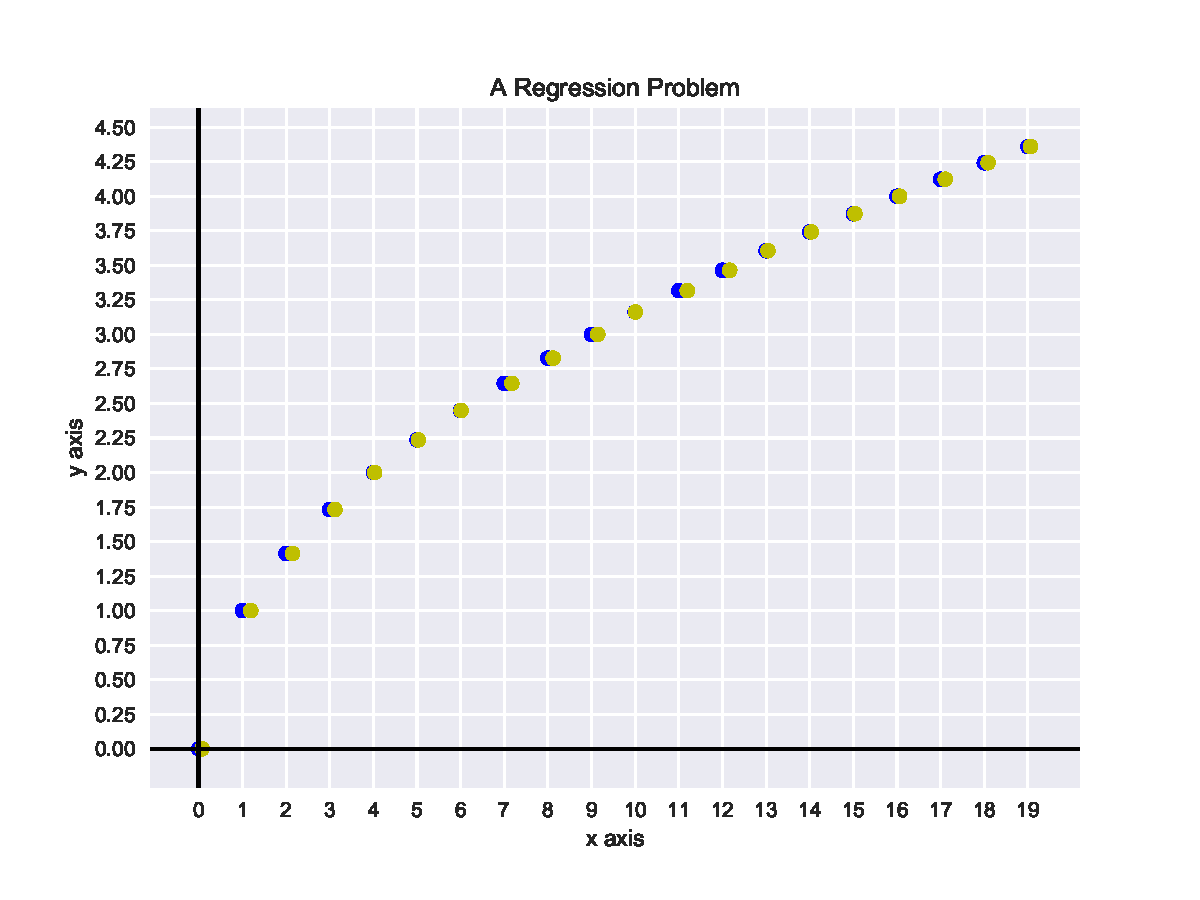
\epsfig{file=Figures/sqrt.pdf, scale=0.8}
\caption{$y = \sqrt{x_1}$, $x_2 = x_1 + \mathtt{noise}$.}
\label{fig:sqrt.pdf}
\end{figure}


\begin{figure}[!th]
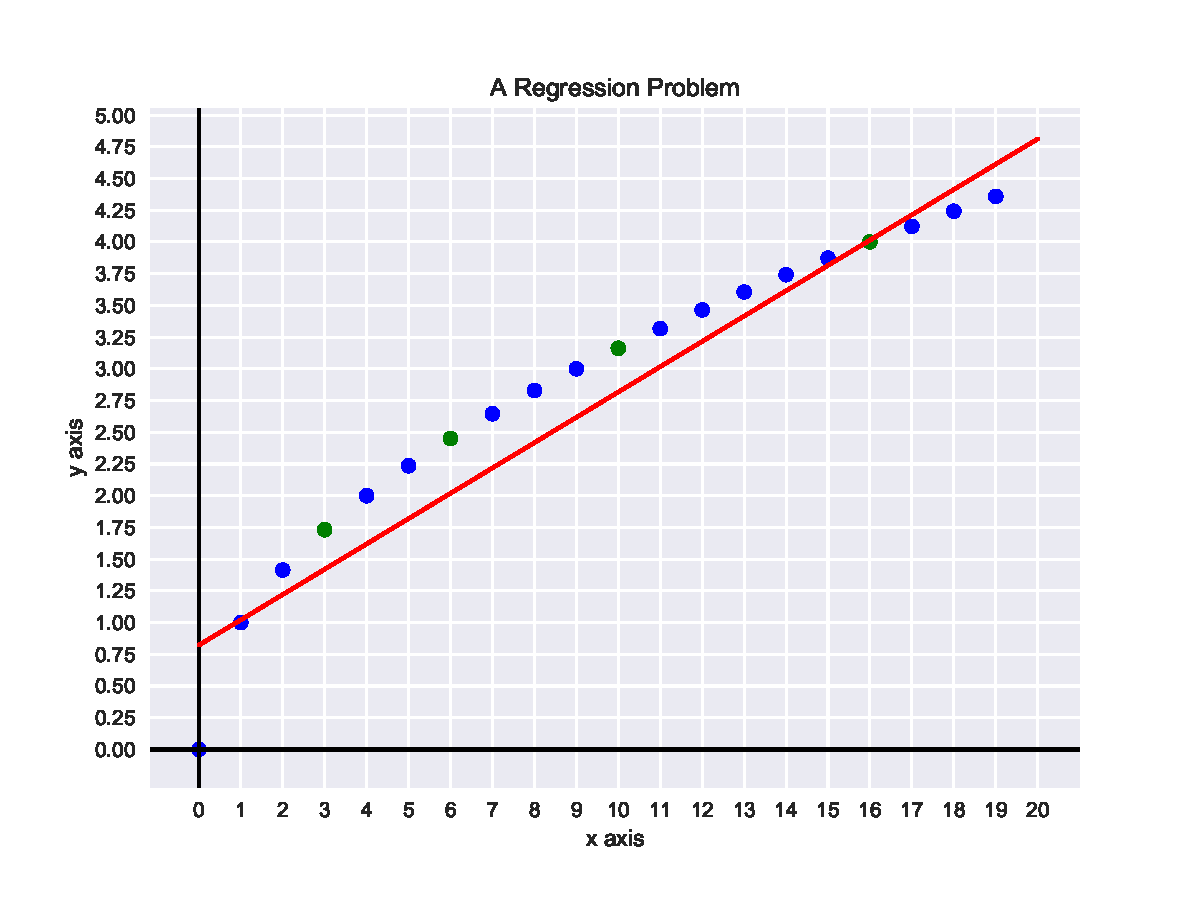
\epsfig{file=Figures/sqrt-linear.pdf, scale=0.8}
\caption{Linear Regression for $y = \sqrt{x_1}$, $x_2 = x_1 + \mathtt{noise}$.}
\label{fig:sqrt-linear.pdf}
\end{figure}

\begin{figure}[!th]
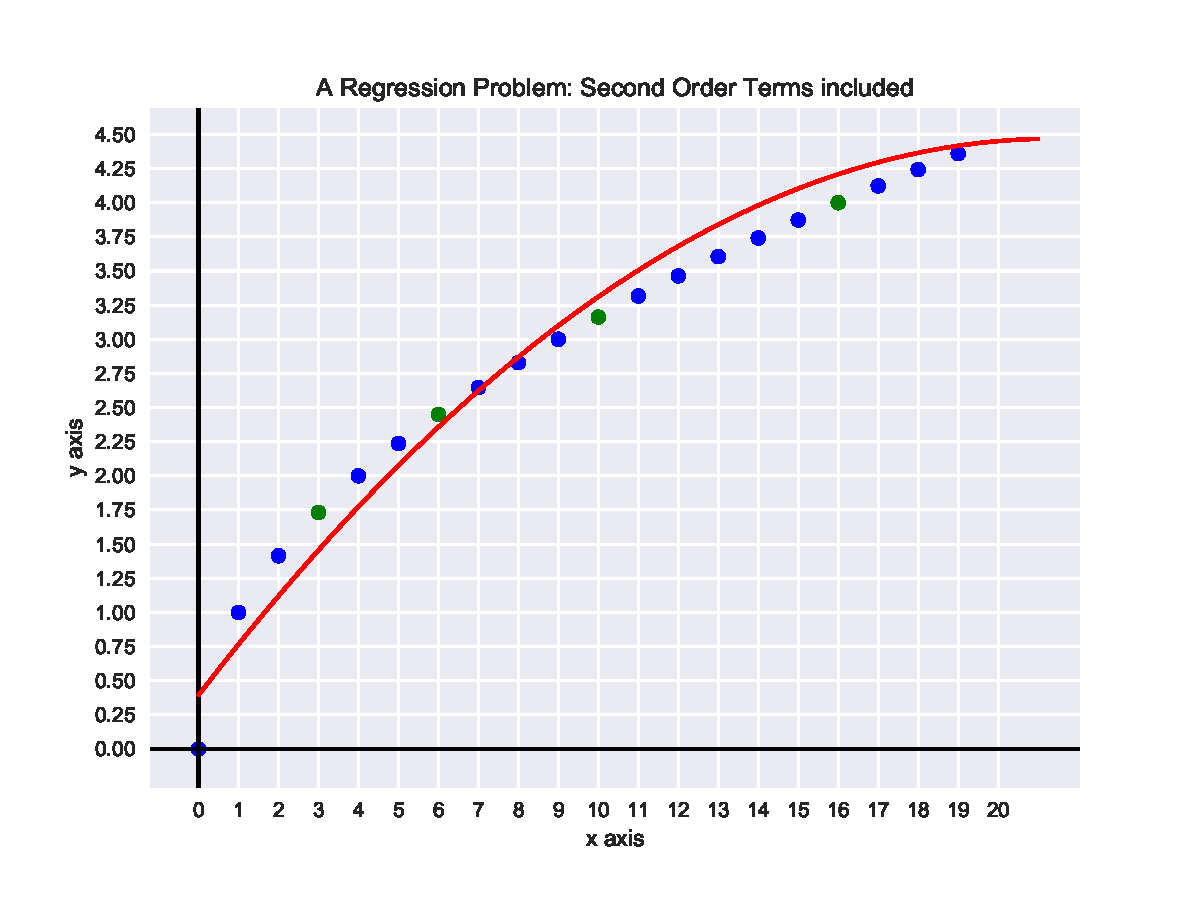
\epsfig{file=Figures/sqrt-quadratic.pdf, scale=0.8}
\caption{Second Order Linear Regression for $y = \sqrt{x_1}$, $x_2 = x_1 + \mathtt{noise}$.}
\label{fig:sqrt-quadratic.pdf}
\end{figure}

Having tried second order terms, we are tempted to go further and try all terms up to the fourth order.
If we do this, the proportion of explained variance on the training set improves to $99.99\%$.  However, on the
test set we get a proportion of explained variance of $96\%$ which, although an improvement, 
is much worse than the explained variance on the training set.
Figure \ref{fig:sqrt-4.pdf} on page \pageref{fig:sqrt-4.pdf} shows the corresponding model.

If we get even bolder and try all terms up to the sixth order, 
the proportion of explained variance on the training set improves to $100\%$.  However, on the
test set we the proportion of explained variance drops of $86.5\%$.  This is called \blue{overfitting}:
\index{overfitting}
Our model is now so complex that it can essentially remember all the training examples it has seen.  However,
it is unable to generalize from these training examples.  Figure \ref{fig:sqrt-6.pdf} on page
\pageref{fig:sqrt-6.pdf} shows the corresponding model.  We see that regression curve gets wiggly, which is
also an indication that we are experiencing overfitting.

\begin{figure}[!th]
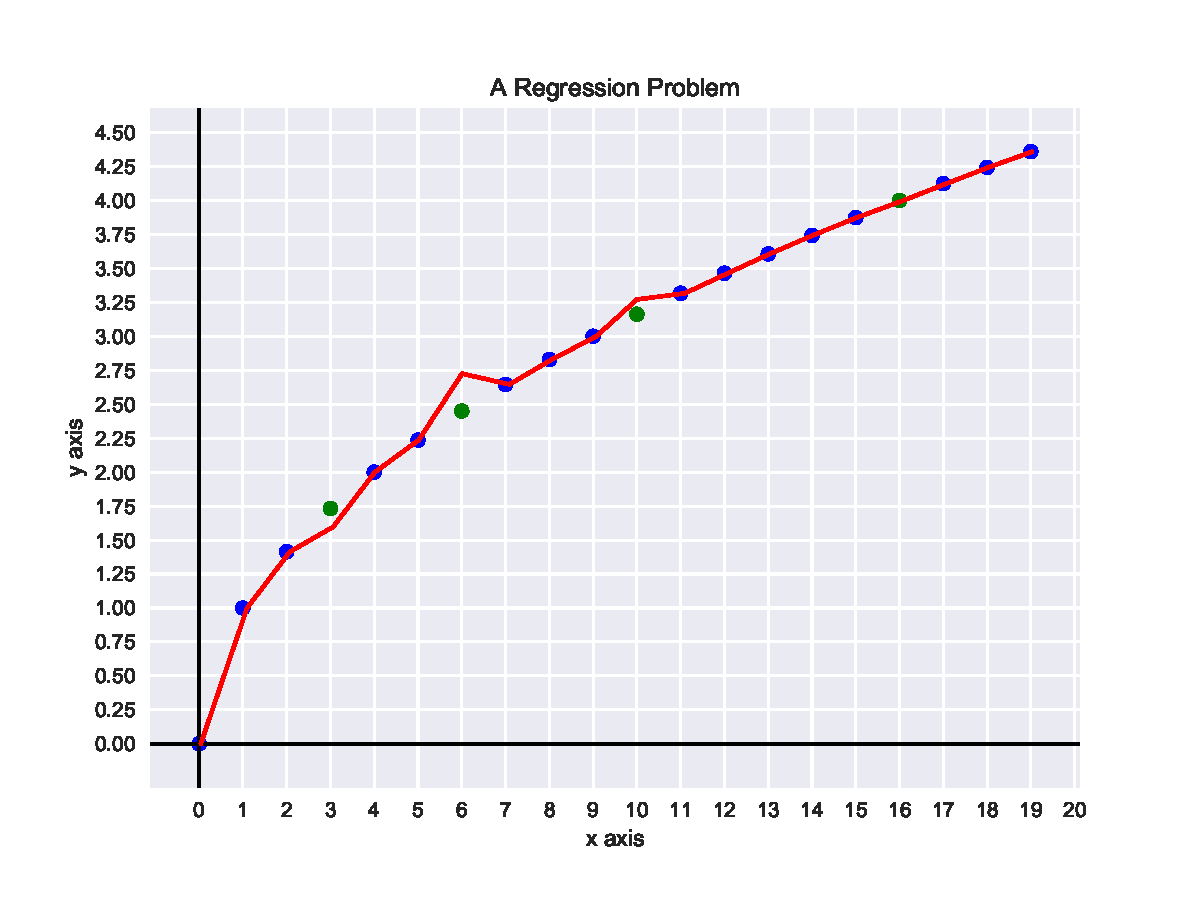
\epsfig{file=Figures/sqrt-4.pdf, scale=0.8}
\caption{Fourth Order Linear Regression for $y = \sqrt{x_1}$, $x_2 = x_1 + \mathtt{noise}$.}
\label{fig:sqrt-4.pdf}
\end{figure}

\begin{figure}[!th]
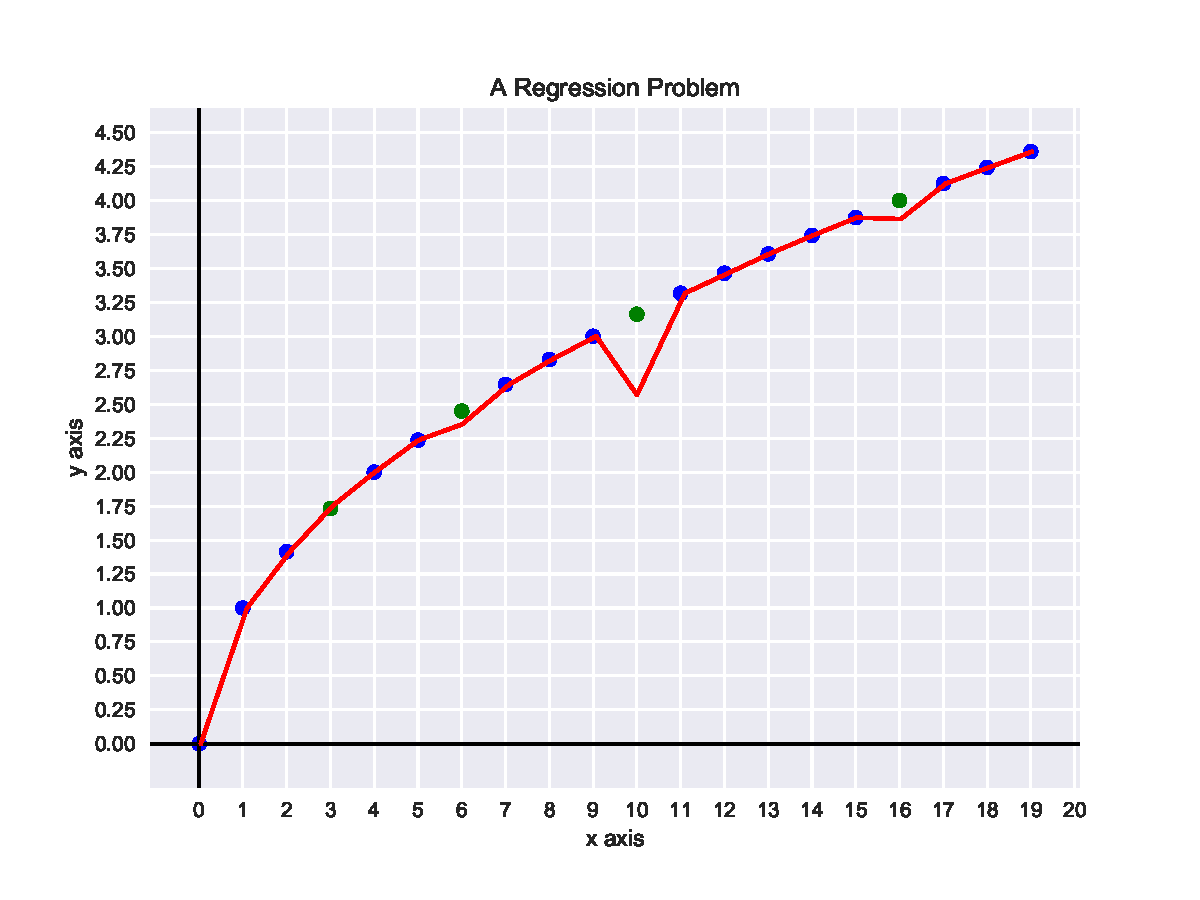
\epsfig{file=Figures/sqrt-6.pdf, scale=0.8}
\caption{Sixth Order Linear Regression for $y = \sqrt{x_1}$, $x_2 = x_1 + \mathtt{noise}$.}
\label{fig:sqrt-6.pdf}
\end{figure}

\section{Ridge Regression}
\index{ridge regression}
In linear regression, our goal is to minimize the mean squared error that has been defined as
\\[0.2cm]
\hspace*{1.3cm}
$
  \ds
  \mathtt{MSE}(\mathbf{w}) =
  \frac{1}{m-1} \cdot \sum\limits_{i=1}^m \Bigl(\bigl(\mathbf{x}^{(i)})^\top \cdot \mathbf{w}  - y^{(i)}\Bigr)^2.
$
\\[0.2cm]
The previous example has shown that sometimes minimizing the mean squared error leads to overfitting.
One way to avoid overfitting is called \blue{ridge-regression}.  Instead of minimizing the mean squared error,
we instead minimize the expression
\\[0.2cm]
\hspace*{1.3cm}
$
  \ds
  \mathtt{RegMSE}(\mathbf{w}) =
  \frac{1}{m-1} \cdot \sum\limits_{i=1}^m \Bigl(\bigl(\mathbf{x}^{(i)})^\top \cdot \mathbf{w}  - y^{(i)}\Bigr)^2
  + \lambda \cdot \mathbf{w}^2.
$
\\[0.2cm]
Here, the parameter $\lambda$ is called the \blue{regularization parameter}.  \index{regularization parameter}
If $\lambda$ is not too small,
then minimizing $\mathtt{RegMSE}(\mathbf{w})$ forces us to find parameters $\mathbf{w}$ that are small.  This
prevents the model from getting to complex and this prevents over-fitting.  Figure \ref{fig:sqrt-6ridge.pdf} on
page \pageref{fig:sqrt-6ridge.pdf} show the model we get when setting $\lambda = 0.05$.  In this case the
proportion of explained variance is $99.97\%$
on the training set and $99.78\%$ on the test set.  This clearly shows that the model does generalize to
example that it has not seen.

The regularization parameter $\lambda$ is a so called \blue{hyper parameter} \index{hyper parameter}
 that is usually determined by
\href{https://en.wikipedia.org/wiki/Cross-validation_(statistics)}{cross  validation}.  This sound complicated,
but actually is very simple:  We split the training set into $k$ parts.  Then we remove one of these parts and
train the model on the remaining $k-1$ parts.  We use the removed part to try to find the best value for our
hyper parameter by trial and error.  We do this for all of the $k$ parts.  In each case we might find a sightly
different optimal value $\lambda_k$.  Finally, we take the mean $\bar{\lambda}$ of all values $\lambda_k$ that
we have found in our $k$ experiments.
Following that we use the complete training set one last time to find a model that uses the value
$\bar{\lambda}$.  It is important to keep the test set untouched while searching for the best value of $\lambda$.




\begin{figure}[!th]
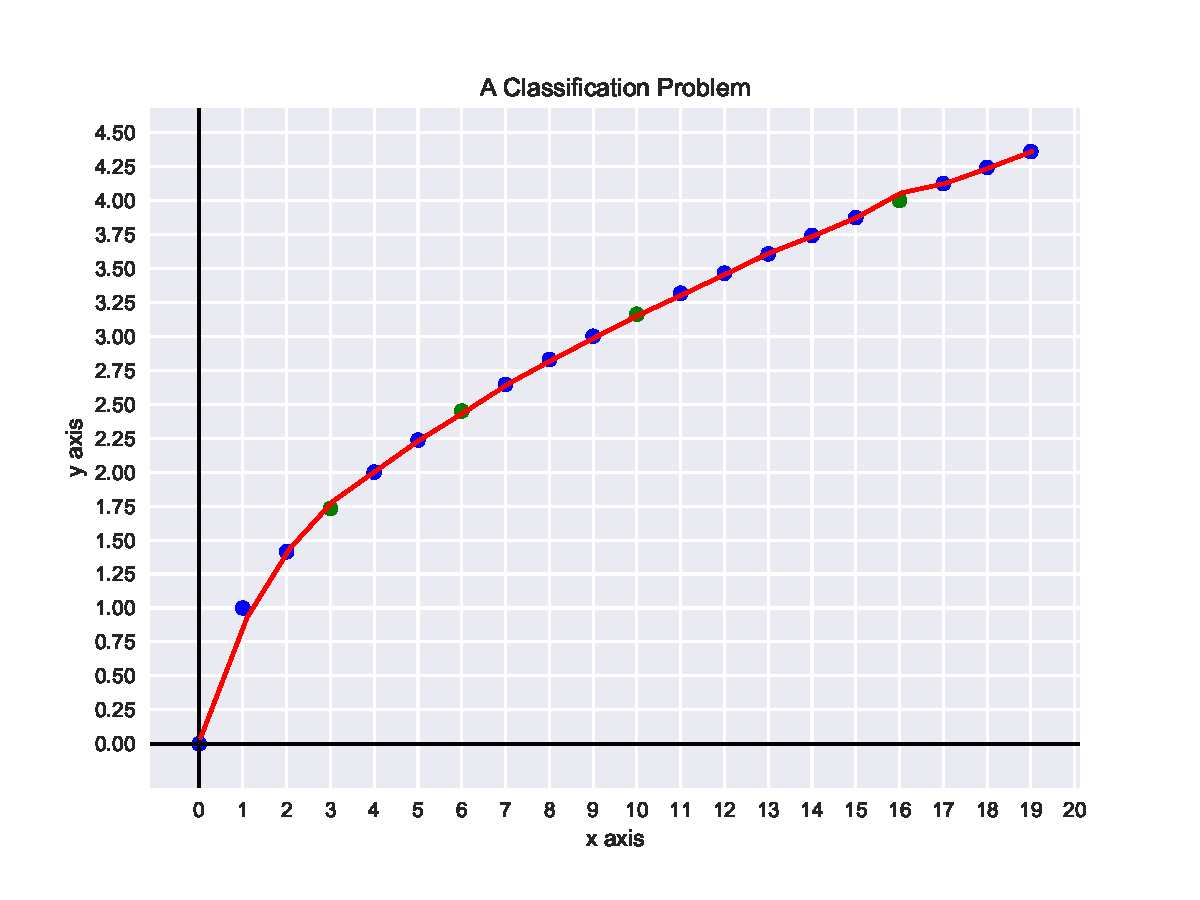
\epsfig{file=Figures/sqrt-6ridge.pdf, scale=0.8}
\caption{Sixth Order Ridge Regression for $y = \sqrt{x_1}$, $x_2 = x_1 + \mathtt{noise}$.}
\label{fig:sqrt-6ridge.pdf}
\end{figure}

\pagebreak


\exercise
The file ``\texttt{trees.csv}'', which is available at
\\[0.2cm]
\hspace*{0.3cm}
\href{https://github.com/karlstroetmann/Artificial-Intelligence/blob/master/Python/trees.csv}{\texttt{https://github.com/karlstroetmann/Artificial-Intelligence/blob/master/Python/trees.csv}},
\\[0.2cm]
contains data about 31 lovely cherry trees from the Allegheny National Forest in Pennsylvania that have fallen
prey to a \href{https://en.wikipedia.org/wiki/The_Texas_Chain_Saw_Massacre}{chainsaw massacre}.  I have taken this data from
\\[0.2cm]
\hspace*{1.3cm}
\href{http://www.statsci.org/data/general/cherry.txt}{\texttt{http://www.statsci.org/data/general/cherry.txt}}.
\begin{enumerate}
\item The first column of this \textsc{Csv} file contains the diameter of these trees at a height of 54 inches above
      the ground.
\item The second column lists the heights of these trees in inches.
\item The third column list the volume of wood that has been harvested from these trees.  This volume is given
      in cubic inches.
\end{enumerate}
Try to derive a model that estimates the volume of the trees from the diameter and the height.
\eox
\pagebreak

\exercise
The file ``\texttt{nba.csv}'', which is available at
\\[0.2cm]
\hspace*{0.3cm}
\href{https://github.com/karlstroetmann/Artificial-Intelligence/blob/master/Python/nba.csv}{\texttt{https://github.com/karlstroetmann/Artificial-Intelligence/blob/master/Python/nba.csv}},
\\[0.2cm]
contains various data about professional basket ball players.
\begin{enumerate}
\item The first column gives the name of the player.
\item The second column specifies the position of the player.
\item The third column lists the height of the player.
\item The fourth column contains the weight of the player.
\item The fifth column shows the age of each player.
\end{enumerate}
To what extend can you predict the weight of a player given his height and his age?
\eox



%%% Local Variables:
%%% mode: latex
%%% TeX-master: "artificial-intelligence"
%%% End:
